\documentclass{article}
\usepackage{graphicx, amsmath, amssymb, mathtools, fancyhdr} % Required for inserting images

\graphicspath{{Images/}}

\setlength{\oddsidemargin}{0in}
\setlength{\textwidth}{6.5in}
\setlength{\topmargin}{-.55in}
\setlength{\textheight}{9in}
\pagestyle{fancy}

\fancyfoot{}
\fancyhead[R]{\thepage}
\fancyhead[L]{MATH 6440}

\newcommand{\res}[1]{\underset{z = #1}{\text{Res}}}


\begin{document}

\begin{center}
    {\huge Approximation Methods HW 4}
    \vspace{0.5cm}

    {\large Michael Nameika}
\end{center}

\begin{itemize}
    \item[\textbf{6.4.1}] Use the method of steepest descent to find the leading asymptotic behavior as $k \to \infty$ of
    \begin{itemize}
        \item[(a)] ${\displaystyle \int_{-\infty}^{\infty}\frac{te^{ik\left(\frac{t^3}{3}+t\right)}}{1+t^4}dt }$
        \newline\newline
        \textit{Soln.} Let $\phi(z) = i\left(\frac{z^3}{3} + z\right)$ and notice $\phi'(z) = i(z^2 + 1) = 0 \implies z = \pm i$ so that $\pm i$ are saddle points of $\phi$. Notice
        \begin{align*}
            \phi(i) &= i\left(-\frac{i}{3} + i\right)\\
            &= -\frac{2}{3}\\
            \phi(-i) &= i\left(\frac{i}{3} - i\right)\\
            &= \frac{2}{3}
        \end{align*}
        and since $\text{Re}(\phi(i)) < 0$, $\text{Re}(\phi(-i)) > 0$, we expect the main contribution of the integral to be near $z = i$. Now, notice
        \begin{align*}
            \phi(z) &= i\left(\frac{(x + iy)^3}{3} + x + iy\right)\\
            &= i\left(\frac{1}{3}x^3 + ix^2y - xy^2 - \frac{1}{3}iy^3 + x + iy\right)\\
            &= -\left(x^2y - \frac{1}{3}y^3 + y\right) + i\left(\frac{1}{3}x^3 - xy^2 + x\right)
        \end{align*}
        so that at $z = i$, the steepest descent contour is given by $\frac{1}{3}x^3 - xy^2 + x = 0 \implies x\left(\frac{1}{3}x^2 - y^2 + 1\right) = 0 \implies x = 0$ or $y^2 - x^2 = 1$. We then deform the contour:

        \begin{center}
            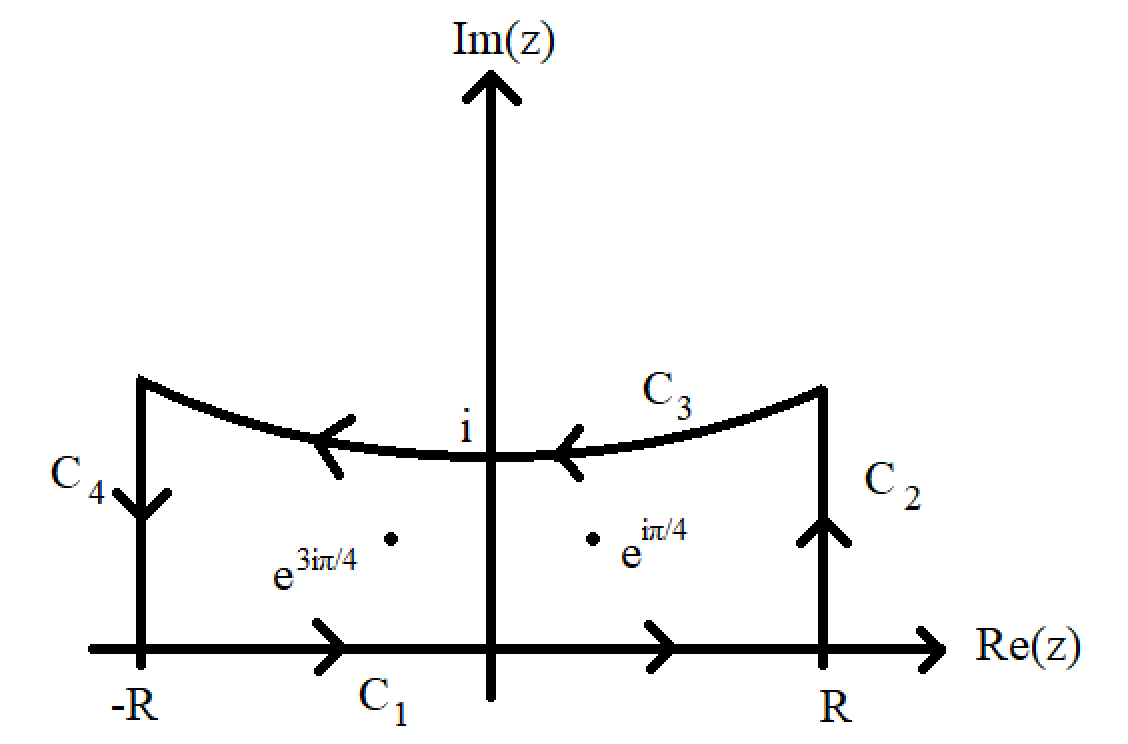
\includegraphics[scale = 0.4]{prob1acontour.PNG}
        \end{center}

        Notice that $z = e^{i\pi/4}$ and $z = e^{3i\pi/4}$ are simple poles of $\frac{z}{1 + z^4}$ since
        \[(1 + z^4) = (z - e^{i\pi/4})(z - e^{3i\pi/4})(z - e^{5i\pi/4})(z - e^{7i\pi/4}).\]
        Further note that the poles at $z = e^{i\pi/4}$ and $e^{3i\pi/4}$ are contained in our deformed contour for sufficiently large $R$, so that by the Residue theorem, we have
        \begin{align*}
            \int_{C_1} + \int_{C_2} + \int_{C_3} + \int_{C_4} &= 2\pi i\left(\res{e^{i\pi/4}}\frac{ze^{ik\left(\tfrac{z^3}{3} + z\right)}}{1 + z^4} + \res{e^{3i\pi/4}}\frac{ze^{ik\left(\tfrac{z^3}{3} + z\right)}}{1 + z^4}\right).
        \end{align*}
        Computing the residues yields
        \begin{align*}
            \res{e^{i\pi/4}}\frac{ze^{ik\left(\frac{z^3}{3} + z\right)}}{1 + z^4} &= \lim_{z \to e^{i\pi/4}}\frac{z(z - e^{i\pi/4})e^{ik\left(\frac{z^3}{3} + z\right)}}{(z - e^{i\pi/4})(z - e^{3i\pi/4})(z - e^{5i\pi/4})(z - e^{7i\pi/4})}\\
            &= \lim_{z \to e^{i\pi/4}}\frac{ze^{ik\left(\frac{z^3}{3} + z\right)}}{(z - e^{3i\pi/4})(z - e^{5i\pi/4})(z - e^{7i\pi/4})}\\
            &= \frac{e^{i\pi/4}e^{ik\left(e^{ik\left(\frac{e^{3i\pi/4}}{3} + e^{i\pi/4}\right)}\right)}}{(e^{i\pi/4} - e^{3i\pi/4})(e^{i\pi/4} - e^{5i\pi/4})(e^{i\pi/4} - e^{7i\pi/4})}\\
            &= -\frac{i}{4}e^{ik\left(\frac{e^{3i\pi/4}}{3} + e^{i\pi/4}\right)}.
        \end{align*}
        Similarly,
        \begin{align*}
            \res{e^{3i\pi/4}}\frac{ze^{ik\left(\frac{z^3}{3} + z\right)}}{1 + z^4} &= \frac{i}{4}e^{ik\left(\frac{e^{i\pi/4}}{3} + e^{i\pi/4}\right)}.
        \end{align*}
        We now argue that the sides of the contour tend to zero as $R \to \infty$. We inspect $C_2$ and note that a similar argument will hold for $C_4$. On $C_2$, parameterize $z = R + iy$ with $0\leq y \leq \sqrt{1 + \frac{R^2}{3}}$. Then
        \begin{align*}
            \int_{C_2} &= i\int_{0}^{\sqrt{1 + \frac{R^2}{3}}}\frac{(R + iy)}{1 + (R + iy)^4}e^{ik\left(\frac{(R + iy)^3}{3} + (R + iy)\right)}dy\\
            &= i\int_0^{\sqrt{1 + \frac{R^3}{3}}} \frac{(R + iy)}{1 + (R + iy)^4}e^{ik\left(\tfrac{1}{3}R^3 + iR^2y - Ry^2 - \tfrac{i}{3}y^3 + R + iy\right)}dy\\
            \implies \left|\int_{C_2}\right| &\leq \int_0^{\sqrt{1 + \frac{R^3}{3}}}\frac{R + 1}{R^4 - 1}e^{-\left(R^2y - \tfrac{1}{3}y^3 + y\right)}dy
        \end{align*}
        where we used $|z| \geq |\text{Re}(z)|$. Now notice for sufficiently large $R$, $R > \sqrt{1 + \frac{R^2}{3}}$ since $\sqrt{1 + \frac{R^2}{3}} \sim R/\sqrt{3}$ as $R \to \infty$. And also note that $R^2y - \frac{1}{3}y^3 + y > 0$ for $0 \leq y \leq R$, hence we can bound the exponential part of the integrand by 1. Hence
        \begin{align*}
            \left|\int_{C_2}\right| &\leq \frac{R(R + 1)}{R^4  - 1}\\
            &\to 0 \hspace{0.4cm} \text{as} \hspace{0.4cm} R \to \infty.
        \end{align*}
        A similar argument shows ${\displaystyle \left|\int_{C_4}\right| \to 0 }$ as $R \to \infty$.
        

        
        
        
        And near $z = i$, notice
        \[\phi(z) \sim -\frac{2}{3} - (z - i)^2.\]
        Then the steepest descent directions are given by 
        \begin{align*}
            \theta &= \frac{2m + 1}{2}\pi + \frac{\pi}{2}, \hspace{0.6cm} m = 0,1\\
            \implies \theta &= 0,\pi.
        \end{align*}
        Thus the top contour is asymptotically equivalent to (after parameterizing with $z = x + i$ and using $\frac{z}{1 + z^4}\sim \frac{i}{2}$ as $z \to i$)
        \begin{align*}
            \int_{C_2} &\sim \frac{i}{2}\int_{-\infty}^{\infty}e^{k\left(-\tfrac{2}{3} - x^2\right)}dz\\
            &= \frac{ie^{-2k/3}}{2}\int_{-\infty}^{\infty}e^{-kx^2}dx\\
            &= \frac{ie^{-2k/3}}{2}\sqrt{\frac{\pi}{k}}.
        \end{align*}
        Finally we have
        \begin{align*}
            &\int_{-\infty}^{\infty} \frac{te^{ik\left(\tfrac{t^3}{3} + t\right)}}{1 + t^4}dt \sim \frac{ie^{-2k/3}}{2}\sqrt{\frac{\pi}{k}} + \frac{\pi}{2}\left(e^{ik\left(\tfrac{e^{i3\pi/4}}{3} + e^{i\pi/4}\right)} - e^{ik\left(\tfrac{e^{i\pi/4}}{3} + e^{3i\pi/4}\right)}\right).
        \end{align*}
        
        \item[(b)] ${\displaystyle \int_{-\infty}^{\infty} \frac{e^{ik\left(\frac{t^5}{5} + t\right)}}{1 + t^2} dt}$
        \newline\newline
        \textit{Soln.} Begin by considering the function $f(z) = \frac{e^{ik\left(\frac{z^5}{5} + z\right)}}{1 + z^2}$. Note that $f(z)$ has simple poles at $z = \pm i$ since $1 + z^2 = (i - z)(i + z)$. Let $\phi(z) = i\left(\frac{z^5}{5} + z\right)$. Then $\phi'(z) = i(z^4 + 1) = 0 \implies z = e^{i\pi/4}, e^{3i\pi/4}, e^{5i\pi/4}, e^{7i\pi/4}$ are saddle points of $\phi$. Note that
        \begin{align*}
            \phi(z) &= i\left(\frac{(x + iy)^5}{5} + x + iy\right)\\
            &= i\left(\frac{1}{5}x^5 + ix^4y - 2x^3y^2 - 2ix^2y^3 + xy^4 + \frac{i}{5}y^5 + x + iy\right)\\
            &= -\left(x^4y - 2x^2y^3 + \frac{1}{5}y^5 + y\right) + i\left(\frac{1}{5}x^5 - 2x^3y^2 + xy^4 + x\right)\\
            \implies \text{Re}(\phi(e^{i\pi/4})) &= -\left(\frac{3}{4\sqrt{2}} + \frac{1}{20\sqrt{2}}\right) < 0\\
            \text{Re}(\phi(e^{3i\pi/4})) &= -\left(\frac{3}{4\sqrt{2}} + \frac{1}{20\sqrt{2}}\right) < 0\\
            \text{Re}(\phi(e^{5i\pi/4})) &= -\left(-\frac{3}{4\sqrt{2}} - \frac{1}{20\sqrt{2}}\right) > 0\\
            \text{Re}(\phi(e^{7i\pi/4})) &= -\left(-\frac{3}{4\sqrt{2}} - \frac{1}{20\sqrt{2}}\right) > 0
        \end{align*}
        which gives that the saddle point contributions will come from $z = e^{i\pi/4}, e^{3i\pi/4}$. Now, at $z = e^{i\pi/4},e^{3i\pi/4}$ we find
        \begin{align*}
            \text{Im}(\phi(e^{i\pi/4})) &= \frac{4}{5\sqrt{2}}\\
            \text{Im}(\phi(e^{3i\pi/4})) &= -\frac{4}{5\sqrt{2}}.
        \end{align*}
        Thus the curves of steepest descent are given by
        \begin{align*}
            \frac{x^5}{5} - 2x^3y^2 + xy^4 + x &= \frac{4}{5\sqrt{2}} \hspace{0.4cm} (z = e^{i\pi/4})\\
            \frac{x^5}{5} - 2x^3y^2 + xy^4 + x &= -\frac{4}{5\sqrt{2}} \hspace{0.4cm} (z = e^{3i\pi/4}).
        \end{align*}
        Deforming the contour gives us

        \begin{center}
            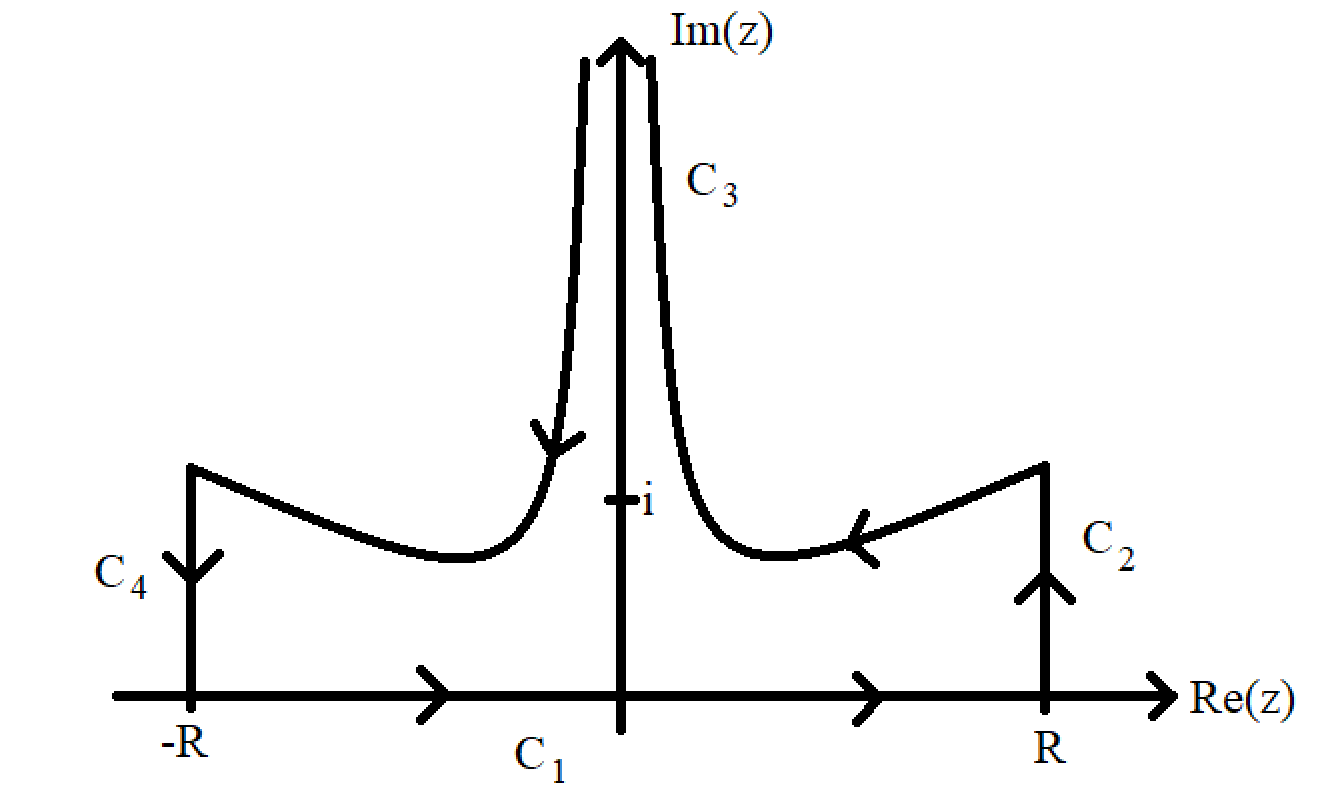
\includegraphics[scale = 0.4]{prob1bcontour.PNG}
        \end{center}

        Thus, by the residue theorem, we have
        \begin{align*}
        \int_{C_1} + \int_{C_2} + \int_{C_3} &= 2\pi i \res{i}\frac{e^{ik\left(\frac{z^5}{5} + z\right)}}{1 + z^2}\\
        &= 2\pi i \lim_{z \to i}\frac{(z - i)e^{ik\left(\frac{z^5}{5} + z\right)}}{(z - i)(z + i)}\\
        &= 2\pi i \lim_{z \to i}\frac{e^{ik\left(\frac{z^5}{5} + z\right)}}{z + i}\\
        &= 2\pi i\frac{e^{ik\left(\frac{i}{5} + i\right)}}{2i}\\
        &= \pi e^{-\frac{6k}{5}}
        \end{align*}
        We now argue that the side contours go to zero as $R \to \infty$. We show $\int_{C_2} \to 0$ as $R \to \infty$ and argue similarly for $C_4$. On $C_2$ parameterize $y = R + iy$. From the parameterization for the steepest descent path, we have
        \begin{align*}
            \frac{R^5}{5} - 2R^3y^2 + Ry^4 + R &= \frac{4}{5\sqrt{2}}\\
            \implies \frac{R^5}{5} - 2R^3s + Rs^2 + R &= \frac{4}{5\sqrt{2}} \hspace{0.4cm} (s = y^2)\\
            \implies s &= \frac{2R^2 \pm \sqrt{4R^4 - 4\left(\frac{R^4}{5} + 1 - \frac{4}{5\sqrt{2}R}\right)}}{2}\\
            \implies y &= \pm\sqrt{R^2 \pm \sqrt{\frac{4}{5}R^4 - 1 + \frac{4}{5\sqrt{2}R}}}.
        \end{align*}
        The upper bound on $y$ is then given as
        \begin{align*}
            y &= \sqrt{R^2 - \sqrt{\frac{4}{5}R^4 - 1 + \frac{4}{5\sqrt{2}R}}}\\
            &\leq R.
        \end{align*}
        Thus, on $C_2$ we have
        \begin{align*}
            \left|\int_{C_2}\right| &\leq \int_0^{\sqrt{R^2 - \sqrt{\frac{4}{5}R^4 - 1 + \frac{4}{5\sqrt{2}R}}}}\left|\frac{R + iy}{1 + (R+iy)^4}e^{ik\left(\frac{(R + iy)^3}{3} + R + iy\right)}\right||idy|\\
            &\leq \int_0^{\sqrt{R^2 - \sqrt{\frac{4}{5}R^4 - 1 + \frac{4}{5\sqrt{2}R}}}} \frac{2R}{R^4 - 1} e^{-k\left(R^2 - \frac{1}{3}y^3 + y\right)}dy.
        \end{align*}
        Note that since $y \leq R$, $y^3 \leq R^3$ and so $R^2 - \frac{1}{3}y^3 + y = R^2 + \frac{2}{3}R^3 > 0$ so we can bound the exponential in the integrand by $1$:
        \begin{align*}
            \left|\int_{C_2}\right| &\leq \frac{2R^2}{R^4 - 1} \to 0 \hspace{0.4cm} \text{as} \hspace{0.4cm} R \to \infty.
        \end{align*}
        A similar argument shows ${\displaystyle \left|\int_{C_4}\right| \to 0 }$ as $R \to \infty$.




        We now wish to find the descent directions near the saddle points on $C_3$. Expanding $\phi(z)$ near $z = e^{i\pi/4}, e^{3i\pi/4}$ gives
        \begin{align*}
            \phi(z) &\approx -\frac{4}{5\sqrt{2}} + i\frac{4}{5\sqrt{2}} - 2e^{3i\pi/4}(z - e^{i\pi/4}) \hspace{0.4cm} \text{near} \hspace{0.4cm} z = e^{i\pi/4}\\
            \phi(z) &\approx -\frac{4}{5\sqrt{2}} - i\frac{4}{5\sqrt{2}} - 2e^{i\pi/4}(z - e^{3i\pi/4}) \hspace{0.4cm} \text{near} \hspace{0.4cm} z = e^{3i\pi/4}.
        \end{align*}
        Thus, the descent directions at $z = e^{i\pi/4}$ are 
        \begin{align*}
            \theta &= \frac{2m + 1}{2}\pi - \frac{5\pi}{8} \hspace{0.4cm} m = 0,1\\
            \implies \theta &= -\frac{\pi}{8}, \frac{7\pi}{8}
        \end{align*}
        and at $z = e^{3i\pi/4}$,
        \begin{align*}
            \theta &= \frac{2m + 1}{2}\pi - \frac{3\pi}{8} \hspace{0.4cm} m = 0,1\\
            \implies \theta &= \frac{\pi}{8}, \frac{9\pi}{8}.
        \end{align*}
        And also note that
        \begin{align*}
            \frac{1}{1 + z^2} &\sim \frac{1}{1 + i} \hspace{0.4cm} \text{near} \hspace{0.4cm} z = e^{i\pi4}\\
            \frac{1}{1 + z^2} &\sim \frac{1}{1 - i} \hspace{0.4cm} \text{near} \hspace{0.4cm} z = e^{3i\pi/4}.
        \end{align*}
        Denote $C_3'$ as the steepest descent curve in the first quadrant and $C_3''$ as the steepest descent curve in the second quadrant. Parameterize $z = re^{-i\pi/8} + e^{i\pi/4}$ on $C_3'$ and $z = re^{i\pi/8} + e^{3i\pi/4}$ on $C_3''$. Then
        \begin{align*}
            \int_{C_3'} &\sim -\frac{e^{-i\pi/8}}{1 + i}\int_{-\infty}^{\infty} e^{k\left(-\frac{4}{5\sqrt{2}} + i\frac{4}{5\sqrt{2}}\right)}e^{-2kr^2}dr \\
            &= -\sqrt{\frac{\pi}{2k}}\frac{e^{-i\pi/8}}{1+i}e^{k\left(-\frac{4}{5\sqrt{2}} + i\frac{4}{5\sqrt{2}}\right)}\\
            &= -\sqrt{\frac{\pi}{k}}\frac{e^{-i\pi/8}}{2e^{i\pi/4}}e^{k\left(-\frac{4}{5\sqrt{2}} + i\frac{4}{5\sqrt{2}}\right)}\\
            &= -\sqrt{\frac{\pi}{k}}\frac{e^{-3i\pi/8}}{2}e^{k\left(-\frac{4}{5\sqrt{2}} + i\frac{4}{5\sqrt{2}}\right)}\\
            \int_{C_3''} &\sim -\frac{e^{i\pi/8}}{1 - i}\int_{-\infty}^{\infty}e^{k\left(-\frac{4}{5\sqrt{2}} - i\frac{4}{5\sqrt{2}}\right)}e^{-2kr^2}dr\\
            &= -\sqrt{\frac{\pi}{2k}}\frac{e^{i\pi/8}}{1 - i}e^{k\left(-\frac{4}{5\sqrt{2}} - i\frac{4}{5\sqrt{2}}\right)}\\
            &= -\sqrt{\frac{\pi}{k}}\frac{e^{i\pi/8}}{2e^{-i\pi/4}}e^{k\left(-\frac{4}{5\sqrt{2}} - i\frac{4}{5\sqrt{2}}\right)}\\
            &= -\sqrt{\frac{\pi}{k}}\frac{e^{3i\pi/8}}{2}e^{k\left(-\frac{4}{5\sqrt{2}} - i\frac{4}{5\sqrt{2}}\right)}.
        \end{align*}
        Thus
        \begin{align*}
            \int_{C_3} &\sim -\sqrt{\frac{\pi}{k}}\left(\frac{e^{3i\pi/8}}{2}e^{k\left(-\frac{4}{5\sqrt{2}} - i\frac{4}{5\sqrt{2}}\right)} + \frac{e^{-3i\pi/8}}{2}e^{k\left(-\frac{4}{5\sqrt{2}} + i\frac{4}{5\sqrt{2}}\right)}\right)\\
            &= -\sqrt{\frac{\pi}{k}}e^{-k\frac{4}{5\sqrt{2}}}\left(\frac{e^{i\left(\frac{4}{5\sqrt{2}}k - \frac{3\pi}{8}\right)} + e^{-i\left(\frac{4}{5\sqrt{2}}k - \frac{3\pi}{8}\right)}}{2}\right)\\
            &= -e^{-\frac{4}{5\sqrt{2}}k}\sqrt{\frac{\pi}{k}}\cos\left(\frac{4}{5\sqrt{2}}k - \frac{3\pi}{8}\right).
        \end{align*}
        Putting it together, we have
        \[\int_{-\infty}^{\infty} \frac{e^{ik\left(\frac{t^5}{5} + t\right)}}{1 + t^2}dt \sim e^{-\frac{4}{5\sqrt{2}}k}\sqrt{\frac{\pi}{k}}\cos\left(\frac{4}{5\sqrt{2}}k - \frac{3\pi}{8}\right) + \pi e^{-\frac{6}{5}k}\]
        
        
    \end{itemize}

    \pagebreak
    \item[\textbf{6.4.4}] In this problem we will find the ``complete" asymptotic behavior of 
    \[I(k) = \int_0^{\frac{\pi}{4}}e^{ikt^2}\tan(t)dt \hspace{0.4cm} \text{as} \hspace{0.4cm} k \to \infty\]
    \begin{itemize}
        \item[(a)] Show that the steepest descent paths are given by 
        \[x^2 - y^2 = C; \hspace{0.4cm} C = \text{ constant}\]
        \textit{Proof:} Let $\phi(z) = iz^2 = i(x + iy)^2 = i(x^2 - y^2 + 2ixy) = -2xy + i(x^2 - y^2)$. Thus at a point $z_0 = x_0 + iy_0$, $\text{Im}(\phi(z_0)) = x_0^2 - y_0^2 := C$. Thus at $z_0$, the steepest descent paths are given by
        \[x_0^2 - y_0^2 = C\]
        where $C$ is constant, as desired.
        \newline\newline

        \item[(b)] Show that the steepest descent/ascent paths that go through $z = 0$ are given by
        \[x = \pm y\]
        and the steepest paths that go through $z = \frac{\pi}{4}$ are given by
        \[x = \pm \sqrt{\left(\frac{\pi}{4}\right)^2 + y^2}\]
        \textit{Proof:} From part (a), the steepest descent path through $z = 0$ is given by
        \begin{align*}
            x^2 - y^2 &= 0\\
            \implies x &= \pm y.
        \end{align*}
        Similarly, the steepest paths through $z = \frac{\pi}{4}$ are given by
        \begin{align*}
            x^2 - y^2 &= \left(\frac{\pi}{4}\right)^2\\
            \implies x &= \pm \sqrt{\left(\frac{\pi}{4}\right)^2 + y^2}
        \end{align*}
        as desired.
        \newline\newline

        \item[(c)] Note that the steepest descent paths in the first quadrant are $C_1 : x = y$ and $C_3 : x = \sqrt{\left(\frac{\pi}{4}\right)^2 + y^2}$. Construct a path $C_2$ as shown in the Figure 6.4.12, and therefore

        \begin{figure}
            \centering
            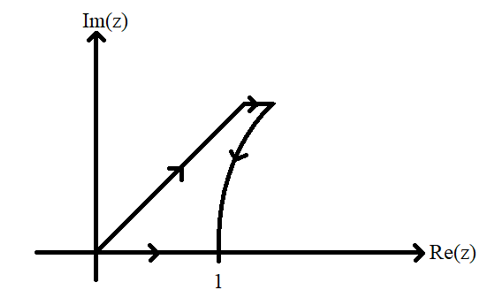
\includegraphics[scale = 0.8]{prob4contour.png}
            \caption{Contour for 6.4.4}
        \end{figure}
        $I(k)$ can be written as $I_1 + I_2 + I_3$ where $I_i$ refers to the integral along contour $C_i$, for $i = 1,2,3$. As $k \to \infty$: show that
        \begin{align*}
            I_1 &\sim \frac{i}{2k} - \frac{1}{6k^2},\\
            I_2 &\sim 0,\\
            I_3 &\sim \frac{-2i}{k\pi}e^{ik(\pi/4)^2}.
        \end{align*}
        \newline\newline
        \textit{Proof:} Note that $\tan(z)e^{ikz^2}$ is holomorphic in and on $C$, so by Cauchy's theorem, we have
        \[\int_C = I_1 + I_2 + I_3.\]
        For $I_1$, we begin by showing $\tan(z) \sim z + \frac{z^3}{3}$ as $z \to 0$. Notice
        \begin{align*}
            \tan(z) &= \frac{\sin(z)}{\cos(z)}\\
            &= \frac{z - \frac{z^3}{3!} + \frac{z^5}{5!} + \mathcal{O}(z^7)}{1 - \frac{z^2}{2!} + \frac{z^4}{4!} + \mathcal{O}(z^6)}\\
            &= \left(z - \frac{z^3}{3!} + \frac{z^5}{5!} + \mathcal{O}(z^7)\right)\left(1 - \frac{z^2}{2!} + \frac{z^4}{4!} + \mathcal{O}(z^6)\right) \hspace{0.4cm} \text{near} \hspace{0.4cm} z = 0\\
            &= z + \left(\frac{z^3}{2} - \frac{z^3}{6}\right) + \left(\frac{5z^5}{24} - \frac{z^5}{12} + \frac{z^5}{120}\right) + \mathcal{O}(z^7)\\
            &= z + \frac{z^3}{3} + \frac{2z^5}{15} + \mathcal{O}(z^7)\\
            \implies \tan(z) &\sim z + \frac{z^3}{3} \hspace{0.4cm} \text{as} \hspace{0.4cm} z \to 0.
        \end{align*}
        Now parameterize $z = re^{i\pi/4}$ and so
        \begin{align*}
            I_1 &\sim e^{i\pi/4}\int_0^{R}re^{i\pi/4}e^{-kr^2}dr + \frac{e^{i\pi/4}e^{3i\pi/4}}{3}\int_0^{R}r^3e^{-kr^2}dr\\
            &\to i\int_0^{\infty}re^{-kr^2}dr - \frac{1}{3}\int_0^{\infty}r^3e^{-kr^2}dr \hspace{0.4cm} \text{as} \hspace{0.4cm} R \to \infty.
        \end{align*}
        Let $u = kr^2$, $du = 2krdr$ so that the above integrals become
        \begin{align*}
            I_1 &\sim \frac{i}{2k}\int_0^{\infty}e^{-u}du - \frac{1}{6k^2}\int_0^{\infty}ue^{-u}du\\
            &= \frac{i}{2k} - \frac{1}{6k^2}
        \end{align*}
        as desired. Now, on $C_2$, parameterize $z = x + iR$ and so
        \begin{align*}
            \int_{C_2} &= \int_R^{\sqrt{\left(\frac{\pi}{4}\right)^2 + R^2}}\tan(x + iR)e^{ik(x + iR)^2}dx\\
            \implies \left|\int_{C_2}\right| &\leq \int_R^{\sqrt{\left(\frac{\pi}{4}\right)^2 + R^2}}|\tan(x + iR)|e^{-2kRx}dx.
        \end{align*}
        We now wish to find an upper bound on $\tan(x + iR)$. Well,
        \begin{align*}
            |\tan(x + iR)| &= \left|-i\frac{e^{ik}e^{-R} - e^{-ix}e^{R}}{e^{ix}e^{-R} + e^{-ix}e^{R}}\right|\\
            &\leq \frac{e^R + e^{-R}}{e^R - e^{-R}}.
        \end{align*}
        Thus
        \begin{align*}
            \left|\int_{C_2}\right| &\leq \frac{e^R + e^{-R}}{e^R - e^{-R}}\int_R^{\sqrt{\left(\frac{\pi}{4}\right)^2 + R^2}} e^{-2kRx}dx\\
            &= -\frac{1}{2kR}\left(\frac{e^R + e^{-R}}{e^R - e^{-R}}\right)\left[e^{-2kRx}\right]\bigg|_R^{\sqrt{\left(\frac{\pi}{4}\right)^2 + R^2}}\\
            &\to 0 \hspace{0.4cm} \text{as} \hspace{0.4cm} R \to \infty.
        \end{align*}
        Finally, on $C_3$, parameterize $x = \sqrt{\left(\frac{\pi}{4}\right)^2 + y^2}$. Then $z^2 = \left(\frac{\pi}{4}\right)^2 + 2iy\sqrt{\left(\frac{\pi}{4}\right)^2 + y^2}$. Let $s = 2iy\sqrt{\left(\frac{\pi}{4}\right)^2 + y^2}$. Then
        \begin{align*}
            z^2 &= \left(\frac{\pi}{4}\right)^2 + is\\
            \implies z &= \sqrt{\left(\frac{\pi}{4}\right)^2 + is}\\
            \implies dz &= \frac{i}{2\sqrt{\left(\frac{\pi}{4}\right)^2 + is}}ds.
        \end{align*}
        Further, $\tan(z) = 1 + 2\left(z - \frac{\pi}{4}\right) + \mathcal{O}\left(\left(z - \frac{\pi}{4}\right)^2\right)$ and so $\tan(z) \sim 1$ as $z \to \frac{\pi}{4}$. Using this, $I_3$ becomes
        \begin{align*}
            I_3 &\sim -\frac{i}{2}\int_0^{\infty}\left(\left(\frac{\pi}{4}\right)^2 + is\right)^{-1/2}e^{ik\left(\left(\frac{\pi}{4}\right)^2 + is\right)}ds\\
            &= -\frac{2i}{\pi}e^{ik(\pi/4)^2}\int_0^{\infty}\left(1 + i\left(\frac{4}{\pi}\right)^2s\right)^{-1/2}e^{-2ks}ds
        \end{align*}
        And near $s = 0$, the binomial expansion gives
        \begin{align*}
            \left(1 + i\left(\frac{4}{\pi}\right)^2s\right)^{-1/2} &= \sum_{n = 0}^{\infty}{-1/2 \choose n}\left[i\left(\frac{4}{\pi}\right)^2s\right]^k\\
            &\sim 1 \hspace{0.4cm} \text{as} \hspace{0.4cm} s \to 0.
        \end{align*}
        Thus
        \begin{align*}
            I_3 &\sim -\frac{2i}{\pi}e^{ik(\pi/4)^2}\int_0^{\infty} e^{-ks}ds\\
            &= -\frac{2i}{\pi k}e^{ik(\pi/4)^2}
        \end{align*}
        as desired.
        
    \end{itemize}

    \pagebreak
    \item[\textbf{6.4.5}] Consider the integral
    \[I(k) = \int_0^1 e^{ikt^3}dt \hspace{0.4cm} \text{as} \hspace{0.4cm} k \to \infty\]
    Show that $I(k) = I_1 + I_2 + I_3$ where as $k \to \infty$:
    \begin{align*}
        I_1 &\sim \frac{e^{i\pi/6}}{3k^{1/3}}\Gamma\left(\frac{1}{3}\right),\\
        I_2 &\sim 0,\\
        I_3 &\sim -\frac{ie^{ik}}{3k} - \frac{2e^{ik}}{9k^2}
    \end{align*}
    and the contour associated with $I_1$ is the steepest descent contour $y = x/\sqrt{3}$ passing through $z = 0$; the contour $I_3$ is the steepest descent contour $x^3 - 3xy^2 = 1$ passing through $z = 1$; and the contour associated with $I_2$ is parallel to the $x-$axis and is at a large distance from the origin.
    \newline\newline
    \textit{Proof:} We consider $I_2$ to be along the path connecting $C_1$ and $C_3$ parallel to the imaginary axis. 
    \begin{center}
        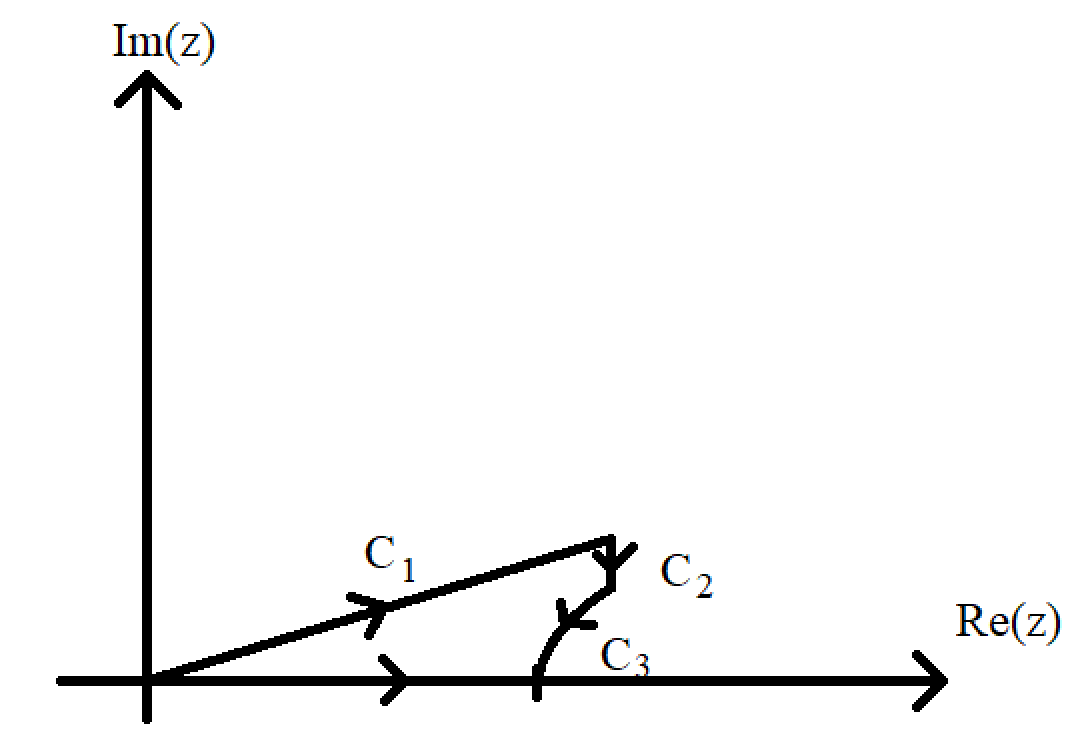
\includegraphics[scale = 0.4]{prob5contour.PNG}
    \end{center}
    On $C_1$, parameterize $z = re^{i\pi/6}$. Then
    \begin{align*}
        \int_{C_1} &= \int_0^{\sqrt{2}/3R} e^{-kr^3}e^{i\pi/6}dr\\
        &= e^{i\pi/6}\int_0^{\sqrt{2}/3R}e^{-kr^3}dr\\
        &\to e^{i\pi/6}\int_0^{\infty} e^{-kr^3}dr\\
        &= \frac{e^{i\pi/6}}{3k^{1/3}}\Gamma\left(\frac{1}{3}\right).
    \end{align*}
    On $I_2$, parameterize $z = R + iy$. Then the lower bound on $y$ is given as $y = \sqrt{\frac{R^3 - 1}{3R}}$. Then 
    \begin{align*}
        I_2 &= i\int_R^{\sqrt{\frac{R^3 - 1}{3R}}}e^{ik(R + iy)^3}dy\\
        \implies |I_2| &\leq \int_{\sqrt{\frac{R^3 - 1}{3R}}}^Re^{-(3R^2y - y^3)}dy\\
        &\leq e^{R^3}\int_{\sqrt{\frac{R^3-1}{3R}}}^R e^{-3R^2y}dy\\
        &= -\frac{e^{R^3}}{3R^2}\left[e^{-3R^2y}\right]\bigg|_{\sqrt{\frac{R^3 - 1}{3R}}}^R\\
        &= -\frac{1}{3R^2}e^{R^3}\left(e^{-3R^3} - e^{-3R^2\sqrt{\frac{R^3 - 1}{3R}}}\right)\\
        &\to 0 \hspace{0.4cm} \text{as} \hspace{0.4cm} R \to \infty.
    \end{align*}

    Now, let $\phi(z) = iz^3 = i(x + iy)^3 = i(x^3 + 3ix^2y - 3xy^2 - iy^3) = -(3x^2y - y^3) + i(x^3 - 3xy^2)$. At $z = 1$, $\text{Im}(\phi(1)) = 1$, so the steepest descent curve at $z = 1$ is given by $x^3 - 3xy^2 = 1$. Solving for $y$ yields $y = \sqrt{\frac{x^3 - 1}{3x}}$. Let $x = 1 + \varepsilon$. For $\varepsilon \ll 1$, notice
    \begin{align*}
        y &= \frac{1}{\sqrt{3}}\left(\frac{(1 + \varepsilon)^3 - 1}{1 + \varepsilon}\right)^{1/2}\\
        &= \frac{1}{\sqrt{3}}\left(\frac{3\varepsilon + 3\varepsilon^2 + \varepsilon^3}{1 + \varepsilon}\right)^{1/2}\\
        &= \frac{1}{\sqrt{3}}\left(\frac{3\varepsilon(1 + \varepsilon)}{1 + \varepsilon} + \frac{\varepsilon^3}{1 + \varepsilon}\right)^{1/2}\\
        &= \sqrt{\varepsilon}\left(1 + \frac{\varepsilon^2}{3(1 + \varepsilon)}\right)^{1/2}\\
        &= \sqrt{\varepsilon}\left(1 + \frac{\varepsilon^2}{3}(1 - \varepsilon + \varepsilon^2 - \mathcal{O}(\varepsilon^3))\right)^{1/2}\\
        &= \sqrt{\varepsilon}\left(1 - \frac{\varepsilon^2}{6} + \mathcal{O}(\varepsilon^3)\right)\\
        \implies y &\sim \sqrt{\varepsilon} \hspace{0.4cm} \text{as} \hspace{0.4cm} \varepsilon \to 0.
    \end{align*}
    Further, expanding $\phi(z)$ around $z = 1$ yields
    \begin{align*}
        \phi(z) &= i\left(1 + 3(z - 1) + 3(z - 1)^2 + \frac{1}{4}(z - 1)^3\right)
    \end{align*}
    parameterize $z = 1 + \varepsilon + i\sqrt{\varepsilon}$, $dz = \left(1 + \frac{i}{2\varepsilon}\right)d\varepsilon$. Using this parameterization for the expansion of $\phi(z)$ above, we find
    \begin{align*}
        \phi(z) &= i\left(1 + 3(\varepsilon + i\sqrt{\varepsilon}) + 3(1 + i\sqrt{\varepsilon})^2 + \frac{1}{4}(\varepsilon + i\sqrt{\varepsilon})^3\right)\\
        &= i\left(1 + 3\varepsilon + 3i\sqrt{\varepsilon} + 3\varepsilon^2 + 6i\varepsilon\sqrt{\varepsilon} - 3\varepsilon + \frac{1}{4}\varepsilon^3 + \frac{3}{4}i\varepsilon^2\sqrt{\varepsilon} - \frac{3}{4}\varepsilon^2 - i\varepsilon^{3/2}\right)\\
        &= i\left(1 + 3i\sqrt{\varepsilon} + 3\varepsilon^2 + 6i\varepsilon\sqrt{\varepsilon} + \frac{1}{4}\varepsilon^3 + \frac{3}{4}i\varepsilon^2\sqrt{\varepsilon} - \frac{3}{4}\varepsilon^2 - i\varepsilon^{3/2}\right)\\
        &\sim i\left(1 + 3i\sqrt{\varepsilon}\right) \hspace{0.4cm} \text{as} \hspace{0.4cm} \varepsilon \to 0.
    \end{align*}
    Thus, using these approximations, we have
    \begin{align*}
        I_3 &\sim -\int_0^{\infty}e^{ik(1 + 3i\sqrt{\varepsilon})}\left(1 + \frac{i}{2\sqrt{\varepsilon}}\right)d\varepsilon\\
        &= -e^{ik}\int_0^{\infty}e^{-3k\sqrt{\varepsilon}}\left(1 + \frac{i}{2\sqrt{\varepsilon}}\right)d\varepsilon\\
        &= -e^{ik}\left(\int_0^{\infty} e^{-3k\sqrt{\varepsilon}}d\varepsilon + i\int_0^{\infty}\frac{1}{2\sqrt{\varepsilon}}e^{-3\sqrt{\varepsilon}}d\varepsilon\right)
    \end{align*}
    letting $u = 3k\sqrt{\varepsilon}$, $du = \frac{3k}{2\sqrt{\varepsilon}}d\varepsilon$ yields
    \begin{align*}
        \implies I_3 &\sim -e^{ik}\left(\frac{2}{9k^2}\int_0^{\infty}ue^{-u}du + \frac{i}{3k}\int_0^{\infty}e^{-u}du\right)\\
        &= -e^{ik}\left(\frac{2}{9k^2} + \frac{i}{3k}\right)\\
        &= -\frac{2e^{ik}}{9k^2} - \frac{ie^{ik}}{3k}
    \end{align*}
    as desired.
    
\end{itemize}

\end{document}
